\documentclass{article}

\usepackage{amsmath} 
\usepackage{subfigure}
\usepackage{caption}
\usepackage{listings}
\usepackage[twocolumn,textwidth=17.31cm,columnsep=.81cm]{geometry}

\usepackage{graphicx}
\usepackage{breqn}
\usepackage{float}
\lstset{ %
 basicstyle=\small,
 breaklines=true,
 }

\begin{document}
\title{Solving Captchas with an OCR system}
\author{Sebastian Agethen, D01944015 \\ Lin Sheng-Ching, R99222030 \\ Jeroen Dhondt, A01922201 }

\onecolumn

\maketitle

\tableofcontents

\twocolumn

\section{Introduction}
\label{sec:intro}

Optical Character Recognition (OCR) has been around for quite some time as a research field in Image Processing. We find this idea interesting, and have thus decided to base our project around OCR. As a new idea and modern application of this topic, we choose to try and solve Captchas. In this introduction we will first introduce the concept of Captchas as well as their motivation and modern day uses, an introduction to the topic of OCR is presented and followed by our motivation to start this project. In Section \ref{sec:implementation} we go in depth over our implementation, covering all different aspects in detail. Next, in Section \ref{sec:evaluation} we sum up our results followed by a discussion. Our conclusions are presented in Section \ref{sec:conclusion}, and the work division is covered in the final Section \ref{sec:division}.

\subsection{Optical Character Recognition}
To start this introduction, we give more insight in the process called OCR. OCR is a term used to describe computer applications with the goal to recognize characters from a (digital) image. As such, these applications have a collection of image processing steps and decision making algorithms that together make it possible to find and correctly identify characters in an image. An example can be seen in Figure \ref{fig:OCRex}. Traditionally, a common application of OCR systems is digitalizing paper resources, for instance old books in libraries or old files in companies. But nowadays a whole new array of applications has risen. Most note-worthy is the extraction of information from images and even video, for instance recognizing license plates on traffic video feeds or analyzing pictures taken by Google Maps to recognize traffic signs, house numbers and others.

\begin{figure} [H]
	\centering
	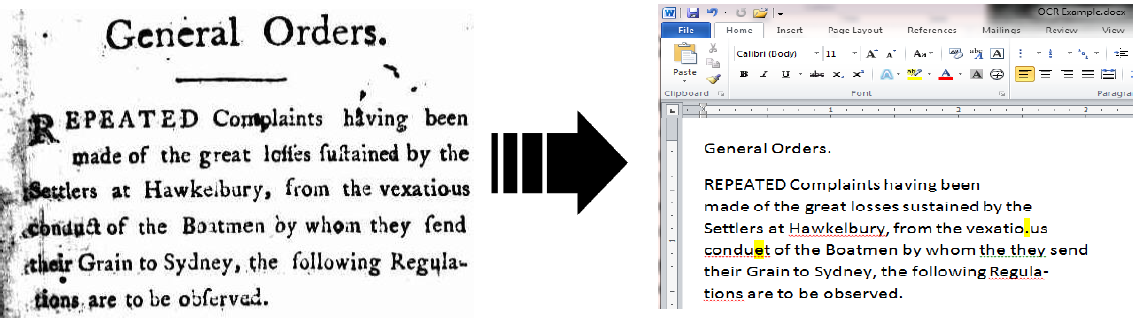
\includegraphics[width=0.5\textwidth]{images/OCRex.PNG}
	\caption{Example of OCR}\label{fig:OCRex}
\end{figure}

\subsection{Captchas}
For our project, we decided to analyze captchas, and ultimately try to solve ('crack') these puzzles. Captchas were invented to solve the problem of so-called 'crawlers' or 'bots' that are found on the web. These automatic programs typically try to spam a website or forum with advertisements or do other unwanted actions. To stop these, captchas were introduced: they are a test to users to prove they are human. These captchas are images with characters hidden in them, in a way that they can be read by humans but are hard to distinguish by a computer. Some examples are shown in Figure \ref{fig:captchas}

\begin{figure}[H]
	\centering
	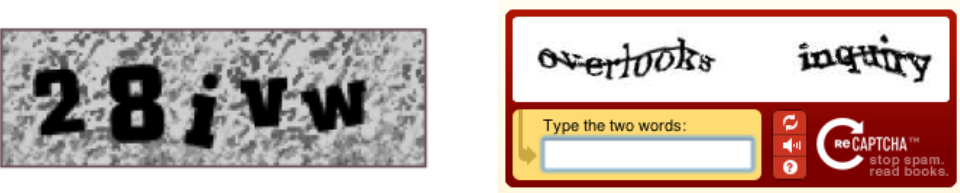
\includegraphics[width=0.5\textwidth]{images/captchas.PNG}
	\caption{Different captchas}\label{fig:captchas}
\end{figure}
 
\subsection{Motivation}
The motivation for our project is to implement an application that can solve captchas, presented as an image file. To get this result, we need to implement two parts: First, a preprocessing of the captcha has to be done. Any distorted elements that obstruct the OCR application from recognizing the characters must be removed. The second and most important part will be the OCR application. Our application must be able to recognize characters found in a given bitmap input image. Due to time constraints, we have only implemented OCR and leave the preprocessing of captchas as future work.

\section{Implementation}
\label{sec:implementation}
We first introduce the structure of our system. In the following sections we then present each step in greater detail.

\subsection{General structure}
Our OCR system runs in two stages, a training phase and a live phase. In the training phase, each of our features is evaluated on a set of 36 bitmaps describing the characters we can recognize. Currently, this encompasses the 26 capital characters of the English alphabet as well as the digits 0 to 9. In the second phase, called live phase, we extract segments from an input file and then compute all features for each segment. Finally, training data and live data are passed together with a weight vector to a clustering method, which can find either the closest or the k-closest matching results.

\subsection{Preprocessing}
A number of Preprocessing tools are necessary to compute the features in Section \ref{sec:features}.

\subsubsection{Quantization}
For implement our quantization method, we first set a threshold value t, and then evaluate the Eq.~\ref{eq:threshold}. If the term $v < t$, we set the pixel $p = 0$, otherwise if $v \geq t$, we set the pixel $p = 1$.
\begin{equation}
v = \sqrt{r^2 + g^2 + b^2}
\label{eq:threshold}
\end{equation}

\begin{figure}
\subfigure[Original B]{

\includegraphics[width=0.5\textwidth]{images/B.pdf}
}
\subfigure[Quantised B]{
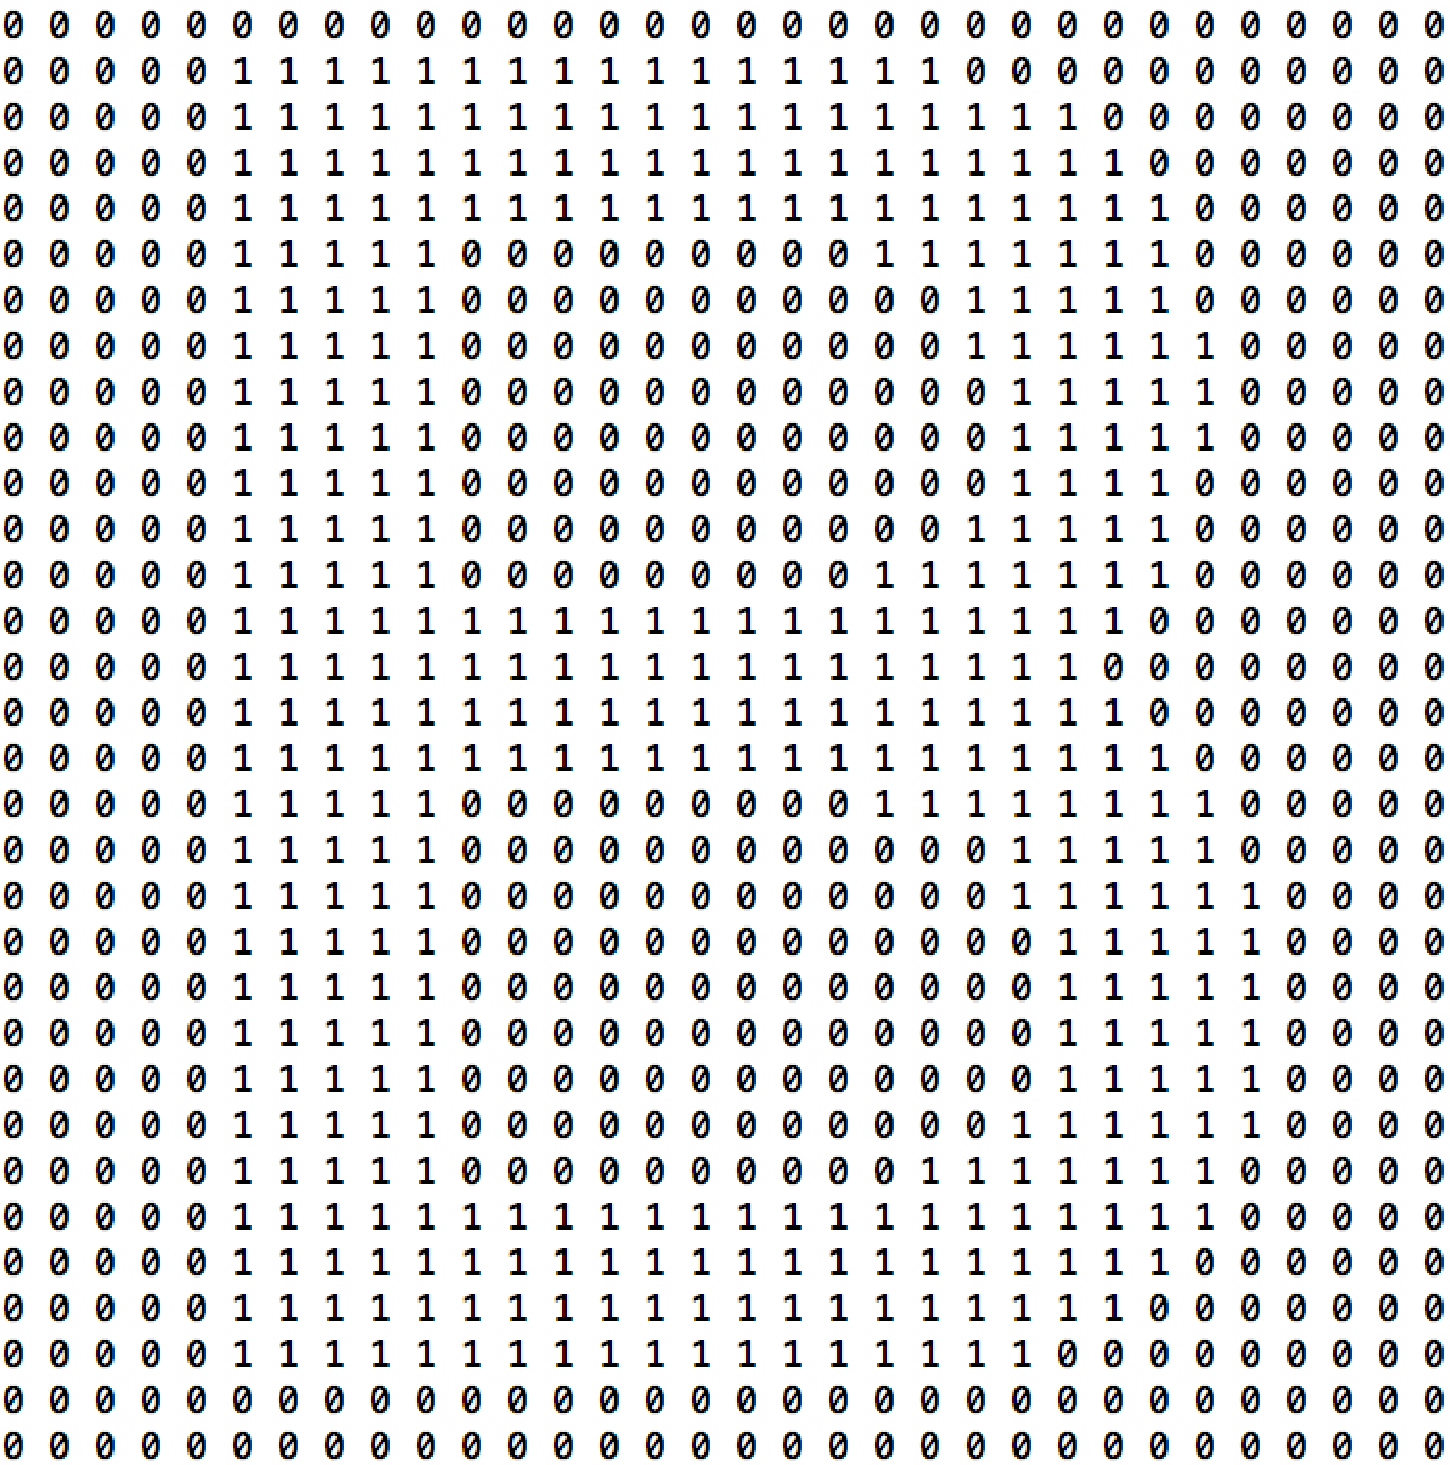
\includegraphics[width=0.5\textwidth]{images/quantised_B.pdf}
}
\caption{Original B v.s. Quantised B}
\end{figure}

\subsubsection{Skeletonization}
After the image is quantized, we repeatedly use the conditional and unconditional mark patterns from \cite{Pratt:2001:DIP:516234} until no further changes occur. Finally, we use a \textit{Bridge} operation to recover the connectivity of the character. Conditional and unconditional mark patterns for Skeletonization can be found in Fig.~\ref{fig:markpatterns1} to \ref{fig:markpatterns3}, while those for the Bridge operation can be found in Fig.~\ref{fig:bridge}.

The comparison of the Skeletonization can be seen in the Fig.~\ref{fig:skeleton}.
\begin{figure}
\subfigure[Quantized B]{
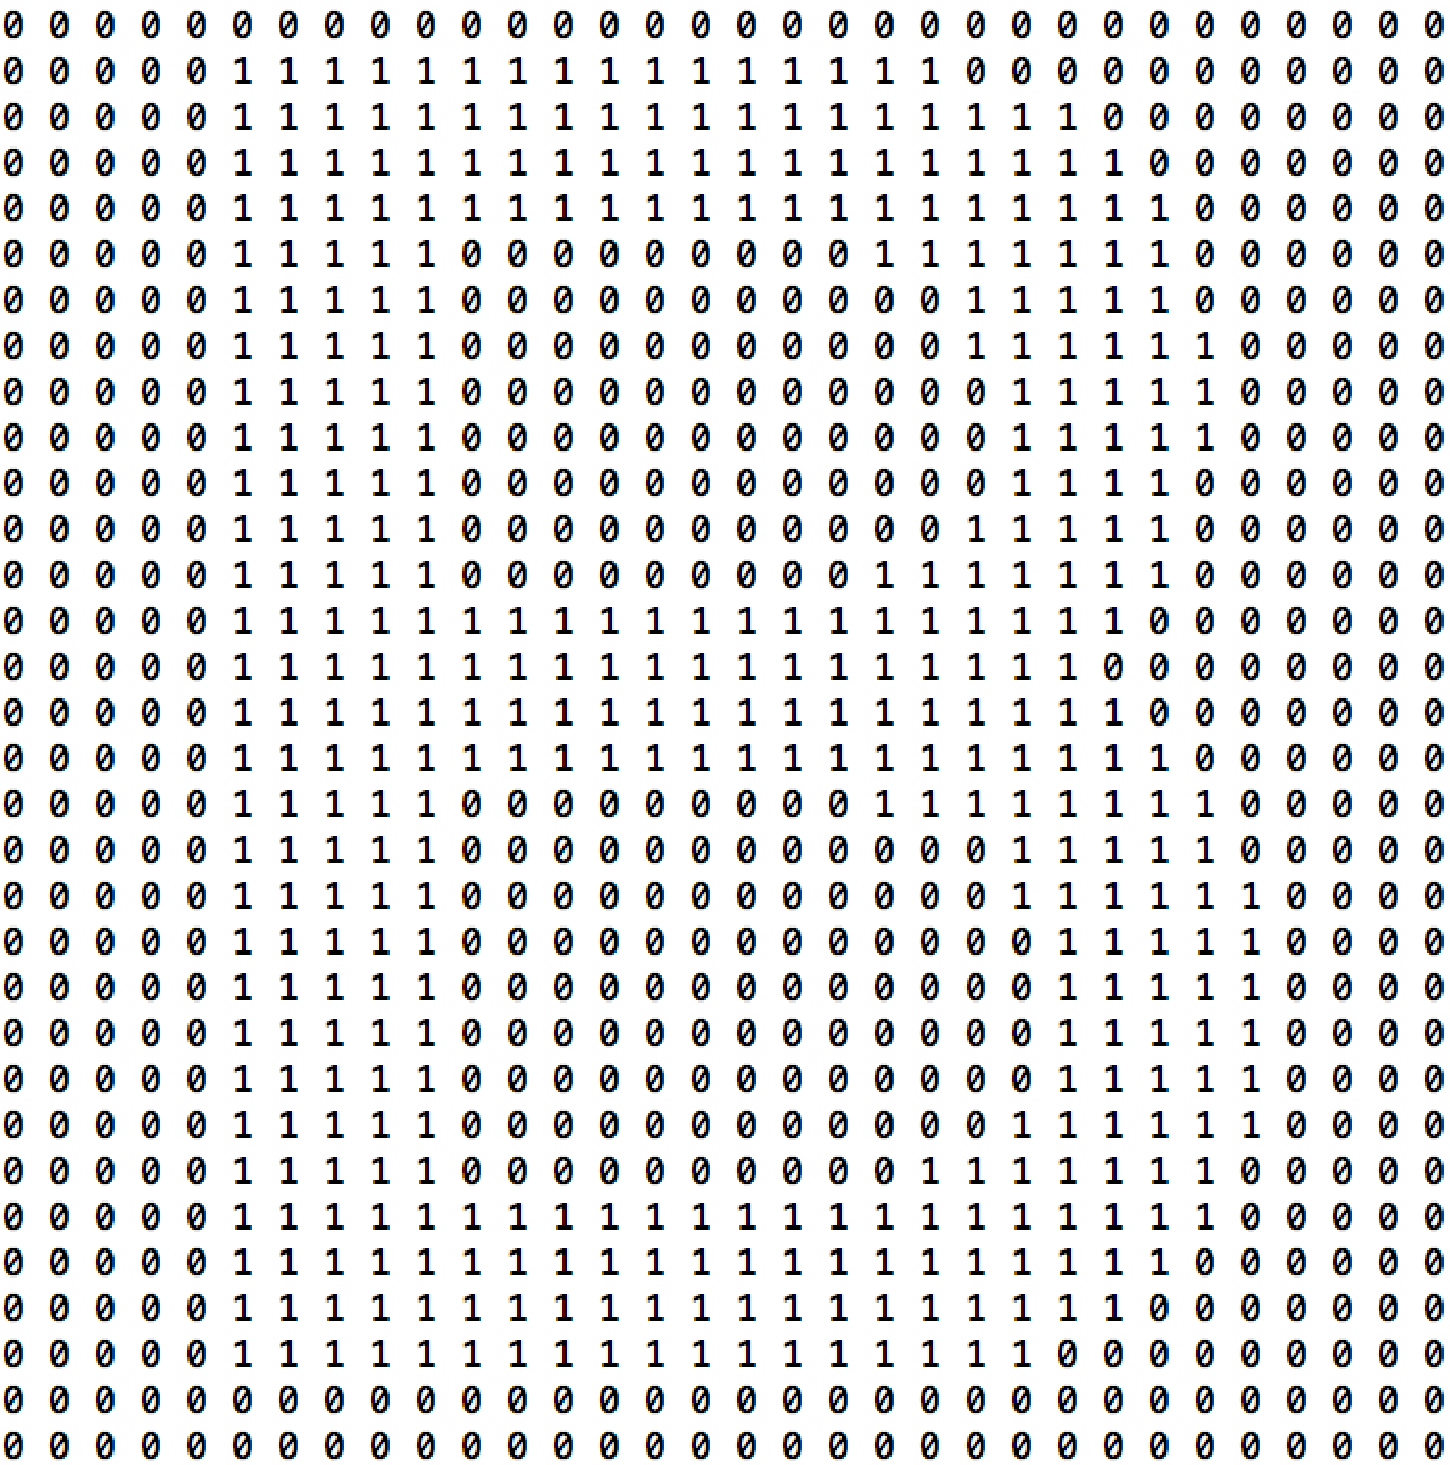
\includegraphics[width=0.5\textwidth]{images/quantised_B.pdf}
}
\subfigure[Skeletonized B]{
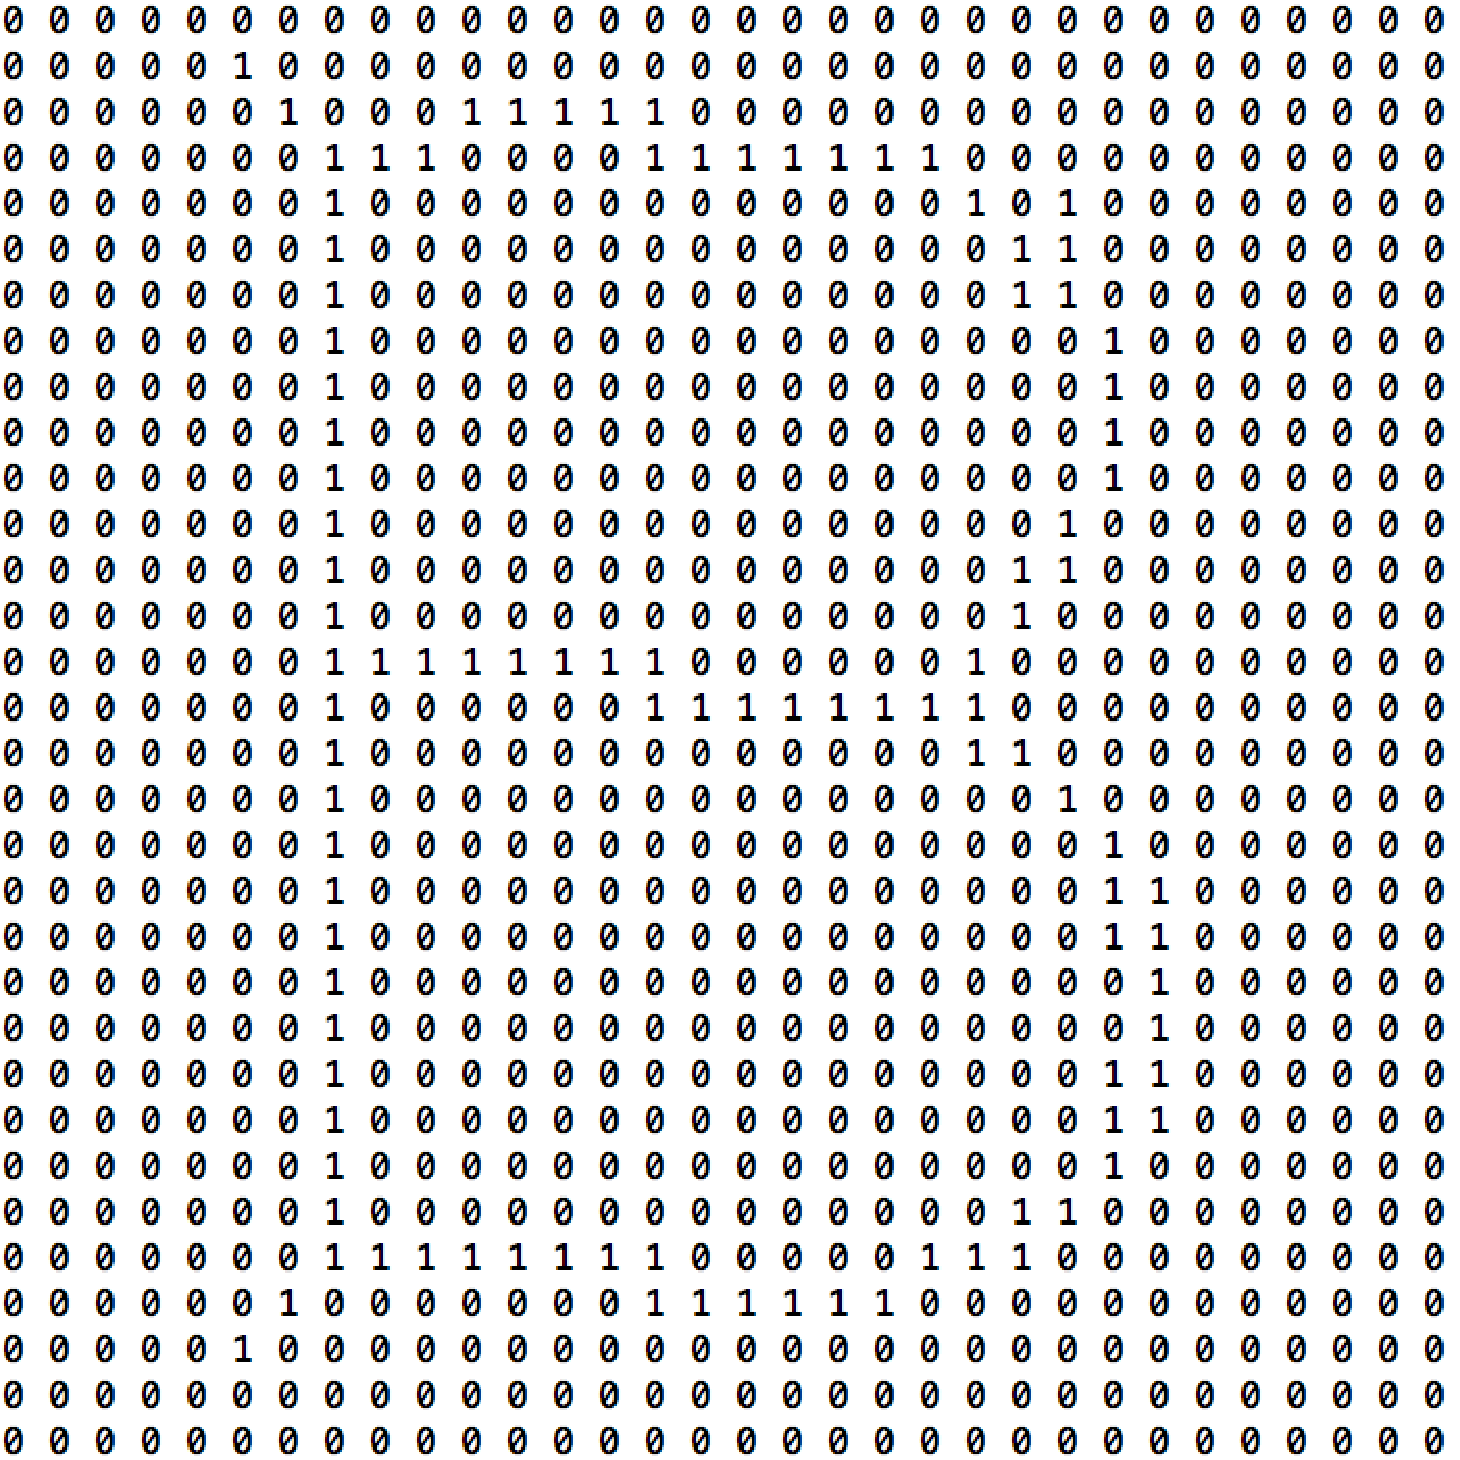
\includegraphics[width=0.5\textwidth]{images/skeletonized_B.pdf}
}
\caption{Quantized B v.s. Skeletonized B}\label{fig:skeleton}
\end{figure}

\subsubsection{Boundary Extraction}
To extract the boundary of a character (in the sense of silhouette, not segmentation), we perform two operations consecutively:
First, we run a single iteration of a shrink algorithm. Formally, the operation is
\begin{equation}
F(j,k) \ominus H(j,k)
\end{equation}
where F(j,k) is the value of original image at position (j,k), and H(j,k) is a mark pattern. In a second step, we then perform a substraction (logically: a XOR) on the original with intermediary result. The results of these operations can be seen in Fig.~\ref{fig:lines} and Fig.~\ref{fig:samples}.

\subsubsection{Segmentation}
Our algorithm to extract single characters from a bitmap can be found in the listing~\ref{lst:boundary}.
\begin{lstlisting}[caption={Segment Extraction algorithm},label={lst:boundary}]
1. Scan the pixel from left to right for each row.
2. When the gradient changes strictly, set the row number as the ceiling of the sentence.
3. After finding the ceiling, keep scanning the pixels. If we find a totally white row, set the row number - 1 as the bottom of the sentence.
4. Scan the pixels of each column from the ceiling to the bottom.
5. When the gradient changes strictly, set the column number as the left boundary of the sentence.
6. After finding the left boundary, scan the pixels from the rightmost pixel to the left, from ceiling to the bottom. As we find a strict gradient of the column, set it as the right boundary.
7. Keep doing the steps 1 ~ 6 until all the input file is scanned.
8. For each sentence, set the left boundary as the left boundary of the first chacter and scan the pixel from ceiling to the bottom, starting from the left.
9. If there is a column totally white, set the column number -1 as the right boundary of the chacter.
10. Keep scanning until a strict gradient occurs. Set the column number as the left boundary of the next chacter.
11. Keep scanning until another strict gradient column is found and the right boundary of the chacter is set.
12. Repeat step 9 ~ 11 until the sentence is totally scanned and scan the next sentence.
\end{lstlisting}

\subsubsection{Orientation}

The following is the derivation of the orientation angle of an object:
We first define the (m,n)th spatial moments as
\begin{multline}
M(m,n)=\frac{1}{J^n K^m}\sum_{j=1}^J\sum_{k=1}^K (x_k)^m (y_j)^n F(j,k)
\end{multline}
where $x_k=k-\frac{1}{2}, y_j=J+\frac{1}{2}-j$ and
\begin{multline}
U(m,n)= \\ \frac{1}{J^n K^m}\sum_{j=1}^J\sum_{k=1}^K \left(x_k-\frac{M(1,0)}{M(0,0)}\right)^m  \left(y_j-\frac{M(0,1)}{M(0,0)}\right)^n F(j,k)
\end{multline}
where $x_k=k-\frac{1}{2}, y_j=J+\frac{1}{2}-j$. Continuing, we find the maximum of the eigen value

\begin{align}
&E^T U E = \Lambda\\
&E=\begin{bmatrix}
 e_{11}&e_{12} \\ 
 e_{21}&e_{22} 
\end{bmatrix}
\\
&\Lambda=\begin{bmatrix}
 \lambda_1&0 \\ 
0 & \lambda_2
\end{bmatrix}
\end{align}
By calculation, 
\begin{multline}
\lambda_1=\frac{1}{2}\left[U(2,0)+U(0,2)\right] + \\ \frac{1}{2}\left[U(2,0)^2+U(0,2)^2-2U(2,0)U(0,2)+4U(1,1)^2\right]^{1/2}
\end{multline}
\begin{multline}
\lambda_2=\frac{1}{2}\left[U(2,0)+U(0,2)\right] - \\ \frac{1}{2}\left[U(2,0)^2+U(0,2)^2-2U(2,0)U(0,2)+4U(1,1)^2\right]^{1/2} 
\end{multline}
\begin{multline}
\rightarrow \theta=\arctan{\left[ \frac{\lambda_M - U(0,2)}{U(1,1)} \right] }
\end{multline}

\subsubsection{Convex Hull}
\label{sec:convexhull}

We define the \textit{Convex Hull} of a character as follows: Given that the input is already quantized to black-and-white, where white is the background, any point that is on a line between any two black points has to be black, too. More formally, this can be expressed as:

\begin{align}
&\forall v_1, \forall v_2 \in \text{B}: v_t \in \text{C},
&v_t = (1-t)v_1 + t v_2, t \in [0,1]
\end{align}
where $B$ is the set of black pixels and $C$ is the Convex Hull. An example can be found in Figure \ref{fig:convex} for the character 'X'.

\begin{figure}
 \centering
  \subfigure[]{
  
\includegraphics{images/X.png}
 }
 \subfigure[]{
  
\includegraphics{images/X_convex.png}
 }
\caption{Convex Hull for the character 'X'. a) Original character, b) Convex Hull of character}
\label{fig:convex}
\end{figure}

\subsection{Features}
\label{sec:features}
In the following we present each feature we used in detail.

\subsubsection{Geometrical features}
\label{sec:geometrical}
%Area, weight center, diameter, etc
Our geometical features consist of area, weight center, average and maximum distance from weight center.
\paragraph{Area}
Calculates the total number of black pixels.

\paragraph{Weight center}
\begin{equation}
F_c=\frac{\sum F(i,j)x_{i,j}}{\sum x_{i,j}}
\end{equation}

\paragraph{Average distance from weight center}
\begin{equation}
d = \sqrt{\frac{\sum_{i,j}(x_{i,j} - F_c)}{\sum_{i,j}x_{i,j}}}
\end{equation}

\paragraph{Maximum distance from weight center}
\begin{equation}
	d_M = MAX(\sqrt{x_{i,j}-F_c})
\end{equation}

\subsubsection{Bays, Lakes and the Euler number}
\label{sec:lakeseuler}
Each character posseses a property called the \textit{Euler number}, which we define as the number of \textit{Connected Components} minus the number of \textit{Lakes}.

In a bitmap that consists of only two colors (e.g., black-and-white), we define a \textit{Lake} to be a connected area which does not reach the borders of the \textit{Convex Hull} (see Section \ref{sec:convexhull}) and is colored with the background color (e.g., white). A related term, the \textit{Bay} is defined to be a connected area of background color that does touch the borders of the \textit{Convex Hull}. The last term is that of a \textit{Connected Component}. For our purposes it will describe any connected area of non-background color (e.g., black). An example for each term is given in Figures \ref{fig:bayslakescomp} a) to d) with the capital character 'A' .

\begin{figure}
 \centering
 \begin{subfigure}[]
  \centering
  
\includegraphics[height=2cm]{images/A_original.png}
  \label{fig:original}
 \end{subfigure}
%
 \begin{subfigure}[]
  \centering
  
\includegraphics[height=2cm]{images/A_bay.png}
  \label{fig:bays}
 \end{subfigure}

 \begin{subfigure}[]
  \centering
  
\includegraphics[height=2cm]{images/A_lake.png}
  \label{fig:lakes}
 \end{subfigure}
%
 \begin{subfigure}[]
  \centering
  
\includegraphics[height=2cm]{images/A_component.png}
  \label{fig:ccomp}
 \end{subfigure}
 \caption{a) Original character, b) 'A' has a single bay (colored red), c) 'A' has one lake, d) 'A' has one Connected Component. Thereby 'A' has Euler number 0 }
 \label{fig:bayslakescomp}
\end{figure}

We compute these features in the following fashion: We sequentially scan the given image for white (Bays and Lakes) or black (Connected Components) pixels. Once such a pixel is found, we then execute a coloring algorithm that recursively visits neighbors of the same color and then colors each visited pixel in a third color (e.g., a greytone). If the coloring algorithm is run on a white pixel, we also determine whether we reached the border of the bitmap during execution by setting a flag \texttt{reachedBorder}. Furthermore, after each instance we increase a counter variable for the corresponding type, e.g., \texttt{numberOfLakes}.

This algorithm visits each pixel at most twice, since the coloring algorithm only visits pixels that have not been colored yet, and therefore requires linear time $O(n)$.

\subsubsection{Line and Circle Components}
Another important property of Latin characters are the number of straight lines and the number of circles within a \textit{Connected Component}. For an example, please refer to Figure \ref{fig:lines}: The character 'A' has zero vertical lines, one horizontal line and zero circles. Note that we currently do not count diagonal lines. However, we reserve this feature for our future work.

\begin{figure}
 \centering
 \subfigure[]{
  
\includegraphics[height=2cm]{images/A_skel_line.png}
 }
 \subfigure[]{
  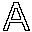
\includegraphics[height=2cm]{images/A_boundary.png}
 }
 
 \caption{a) In Red: Skeleton of 'A' having one horizontal line, b) Boundary Extraction: Two horizontal lines}
\label{fig:lines}
\end{figure}

We use a very simple method to count straight lines: We first search a pixel that is not of background color. Once it is found, we then visit the next pixel in one direction recursively and thereby determine the length of a possible line. For example, to compute horizontal lines and given that the current pixel is located at (x,y), we visit (x+1,y), (x+2,y) and so on until a different color is encountered. We then count the scan as a line if its length meets a predetermined threshold.

A major issue with this algorithm arises when lines have a thickness of more than one pixel: In that case, for varying sizes of characters, varying number of lines would be found! It is therefore imperative to first do preprocessing. We suggest to use either \textit{Skeletonization} or \textit{Boundary Extraction}. When using \textit{Skeletonization}, each line of a character is shrunk to a thickness of 1, enabling easy parsing. When using \textit{Boundary Extraction} however, two lines are (usually) created. In our implementation, we have used \textit{Boundary extraction}.

We can also count the number of circles in a character. To do this, we find a \textit{Lake} (see Sec.~\ref{sec:lakeseuler}) and evaluate the following formula:
\begin{equation}
C_0 = \frac{4\pi A_0}{P_0^2}
\end{equation}

where $A$ is the area of the Lake and $P$ is the \textit{Perimeter}, i.e., the number of neighboring black pixels.

\subsubsection{Shape Context}
We include a method proposed by Belongie et al. \cite{Belongie00shapecontext:} as a feature: Shape Descriptors. A Shape Descriptor is a single value that describes how similar two shapes are, where a value of zero implies that two shapes are identical, whereas rising positive values show differences. 

\begin{figure}
 \centering
 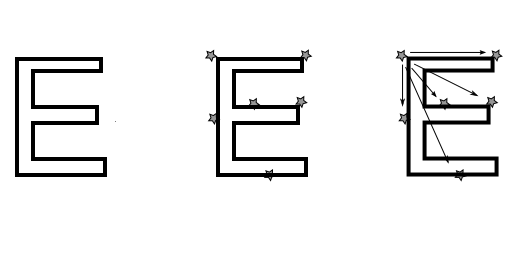
\includegraphics[width=8cm]{images/samples.png}
 \caption{Sampling process: Left: Perform Boundary Extraction, Center: Choose a fixed number of random samples, Right: Compute log-distances between samples}
 \label{fig:samples}
\end{figure}

The authors of the paper construct this value by sampling a picture, computing the distances between samples and then creating a histogram for each sample. When comparing two shapes, the Chi-Square distance 

\begin{displaymath}
C_S = \frac{1}{2} \sum\limits^K_{k=1} \frac{\left[g(k) - h(k)\right]^2}{g(k)+h(k)}
\end{displaymath}

is computed for each pair of histograms of shape A (g in the formula above) with histograms of shape B (h). This results in $n^2$ values! The suggested solution is to find a bipartite matching between samples of shape A and B and then compute the sum of all matched chi-square distances.

Belongie et al. also present a further method to determine orientation in their paper, which we have not implemented.

\subsection{Decision mechanism}
Once every feature has been evaluated on all segments, we need to decide which character a segment resembles. In our system, we use a simple clustering algorithm.

\subsubsection{Weight vector}
An important point to notice is that above features are not normalized. The \textit{Euler number} of a character may range between -1 and 1, while the total black area of a segment may easily have ~300 pixels for letter of font size 32. Normalizing all values improves results greatly. However, another problem occurs: In reality, the Euler number distinguishes a character far more than the area. E.g., we would like to \textbf{weigh} the Euler number higher than the area. To achieve this, we must therefore include a weight-vector. 

\subsubsection{Clustering}

Once this is done, the clustering algorithm is very straightforward: For each segment a vector is created, where each dimension of the vector resembles another feature. Each component of a vector is furthermore multiplied by the corresponding entry in the weight-vector. 

We then choose the vectors found in our training phase to be the cluster centroids. For all other vectors, namely those found in the live phase, we compute the distances to all cluster centroids and then assign it to the closest centroid. The advantage of this method over, e.g., a decision tree is that we can also support k-next-neighbor request, which is useful for post-processing. As we currently do not do any post-processing, we keep this matter for future work.

\section{Experimental Results}
\label{sec:evaluation}
We evaluate our program on the text seen in Figure \ref{fig:input}. The text contain Capitals from the English alphabet as well as the digits 0 to 9.
%\begin{lstlisting}[caption={Input for our evaluation},label={lst:input}]
%ABCDEFGHIJKLMNOPQRSTUVWXYZ0123456789
%AN APPLE A DAY KEEPS THE DOCTOR AWAY
%\end{lstlisting}

\begin{figure}[ht]
 
\includegraphics[width=8cm]{images/demo.png}
 \caption{Input Bitmap for our evaluation}
 \label{fig:input}
\end{figure}

\begin{lstlisting}[caption={Result of our evaluation},label={lst:output}]
Detected: 
ABZDEFDHG2SLNNORORETKXQWYZD5ZB4ZB5BB
Diff:
  C   G IJK M  PQ S UVWX  0123 56789
(22 Errors)

Detected:
ANARRLEADAYSEERETHEDOZTORAQAY
Diff:
   PP      K  PS     C    W  
(7 Errors)
\end{lstlisting}

The output of our OCR system can be seen in Listing \ref{lst:output}. From the total of 65 characters, we incorrectly recognized 29, giving an overall error-ratio of 44.6\%.
We notice that with our current features, the recognition is far better for alphabetical characters than for numbers. From the ten digits only one was correctly identified (error ratio: 90\%), while of the 55 alphabetical characters 35 were correctly identified (error ratio: 36.3\%). 


We also remark that the execution time of our system depends strongly on the number of samples chosen in the \textit{Shape Descriptor} feature. Currently, we use 50 points per segment, which is only half of the proposed number of samples in \cite{Belongie00shapecontext:}. Our demo of 65 characters executed in 0.9646s on a 2.4 GHZ machine.

\subsection{Discussion}
We now discuss the known flaws of our system leading to the low recognition rate above. First of all, some of the features are not well implemented resulting in incorrect values, e.g., our Number of Bays feature. The problem here is that during the computation of the Convex Hull some pixels are falsely included. These pixels then form small Bays that distort our results.

Another problem we met can be revealed from closer study of Fig.~\ref{fig:input}: Notice that the spacing between each character is quite wide. If this is not the case, it may happen that two characters are joined during segmentation. One problem is that characters may overlap, another one is the quantization. Characters in the bitmap are not necessarily black-and-white, but diffuse. It is therefore important to find a good quantization threshold: Is the threshold too high, characters maybe joined due to diffusion. Is the threshold too low, some characters might be split up, especially for small font sizes.

Finally, we also note that adjusting the weights is critically important for a good result. This issue is a keypoint for any future work on this project.

\section{Conclusion}
\label{sec:conclusion}
When we look at our results of the OCR application, we see that some improvements are needed if we want the program to work perfectly. The error rate should be reduced significantly, and this can be tried by different approaches. We can do this by increasing the test phase, using more variations as input for our program. Different, and more decisive features can be implemented, further decreasing the error rate. It is questionable though that very similar characters like 0 and D can ever be 100\% correctly recognized. To achieve this, we can optimize the digitization process of text input even further by implementing a dictonary. This can be seen as a 'second opinion' on the decision made by our application. If the OCR system is in doubt about a character, we can lookup possible combinations in the dictionary and pick the most plausible one.

However, we can conclude that OCR is a very possible application (as has been proved by commercial applications): letters and numbers can be recognized based on their characteristics and in very reasonable time. This observation has lead to a series of applications found nowadays in our daily life. With the increase of computation power and portability of our devices, we can only predict these applications to become even more popular.

\section{Division of Labor}
\label{sec:division}
\begin{tabular}{|l|l|}
 \hline
 Sebastian Agethen & Program Framework, Decision Clustering, \\
  & Features: Lakes, Euler number, \\
 & Lines and Circles, Shape Coefficient\\
\hline
 Lin Sheng-Ching & Extraction of characters, \\
 &  skeletonization of characters\\
  & geometrical features (Sec.~\ref{sec:geometrical}), \\ & orientation \\
\hline
 Jeroen Dhondt & Project Proposal, Bays, \\
 & Presentation/Final Report: Introduction, \\
 & Motivation, Conclusion\\
\hline
\end{tabular}


\begin{figure*}[hb]
 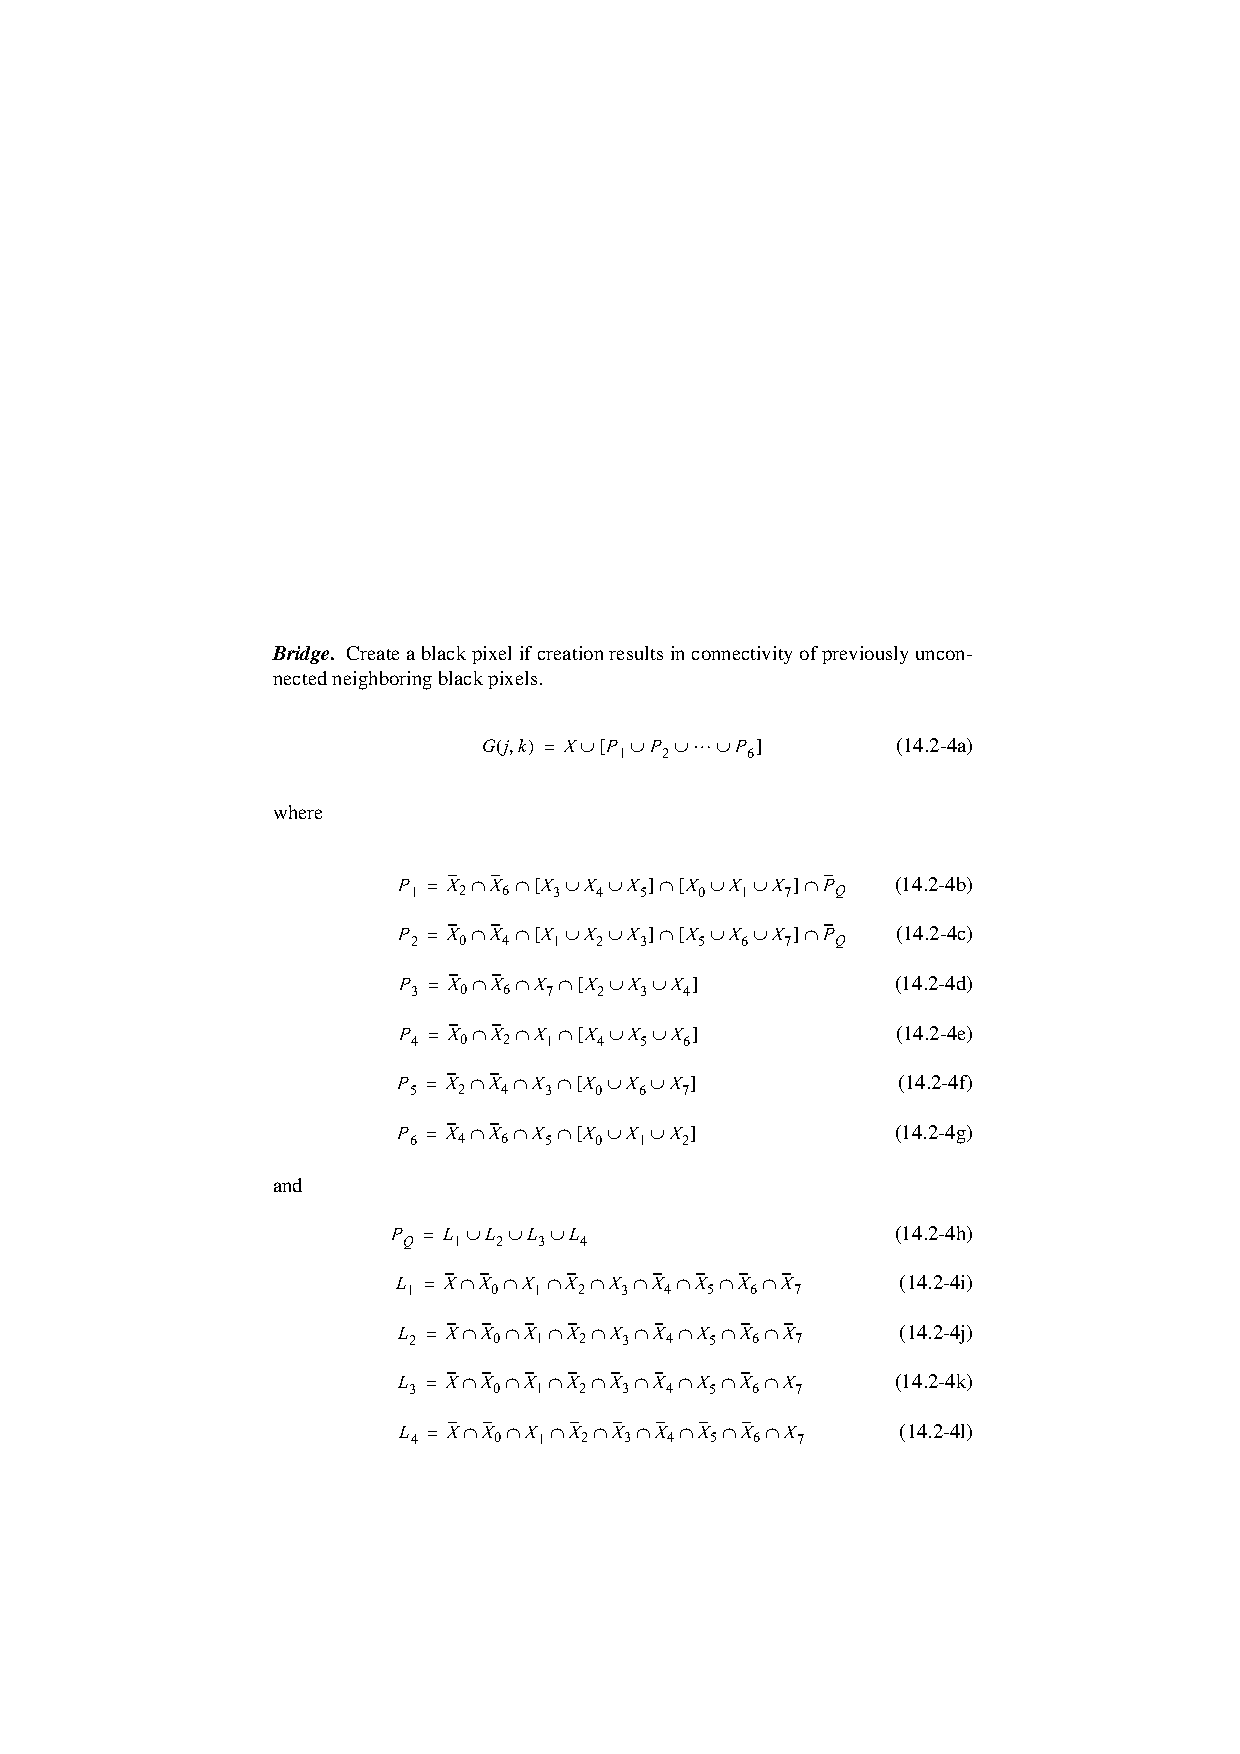
\includegraphics{images/bridge.pdf}
 \caption{Conditions for Bridging a Pixel, taken from \cite{Pratt:2001:DIP:516234}, p. 406}
 \label{fig:bridge}
\end{figure*}

\begin{figure*}[hb]
 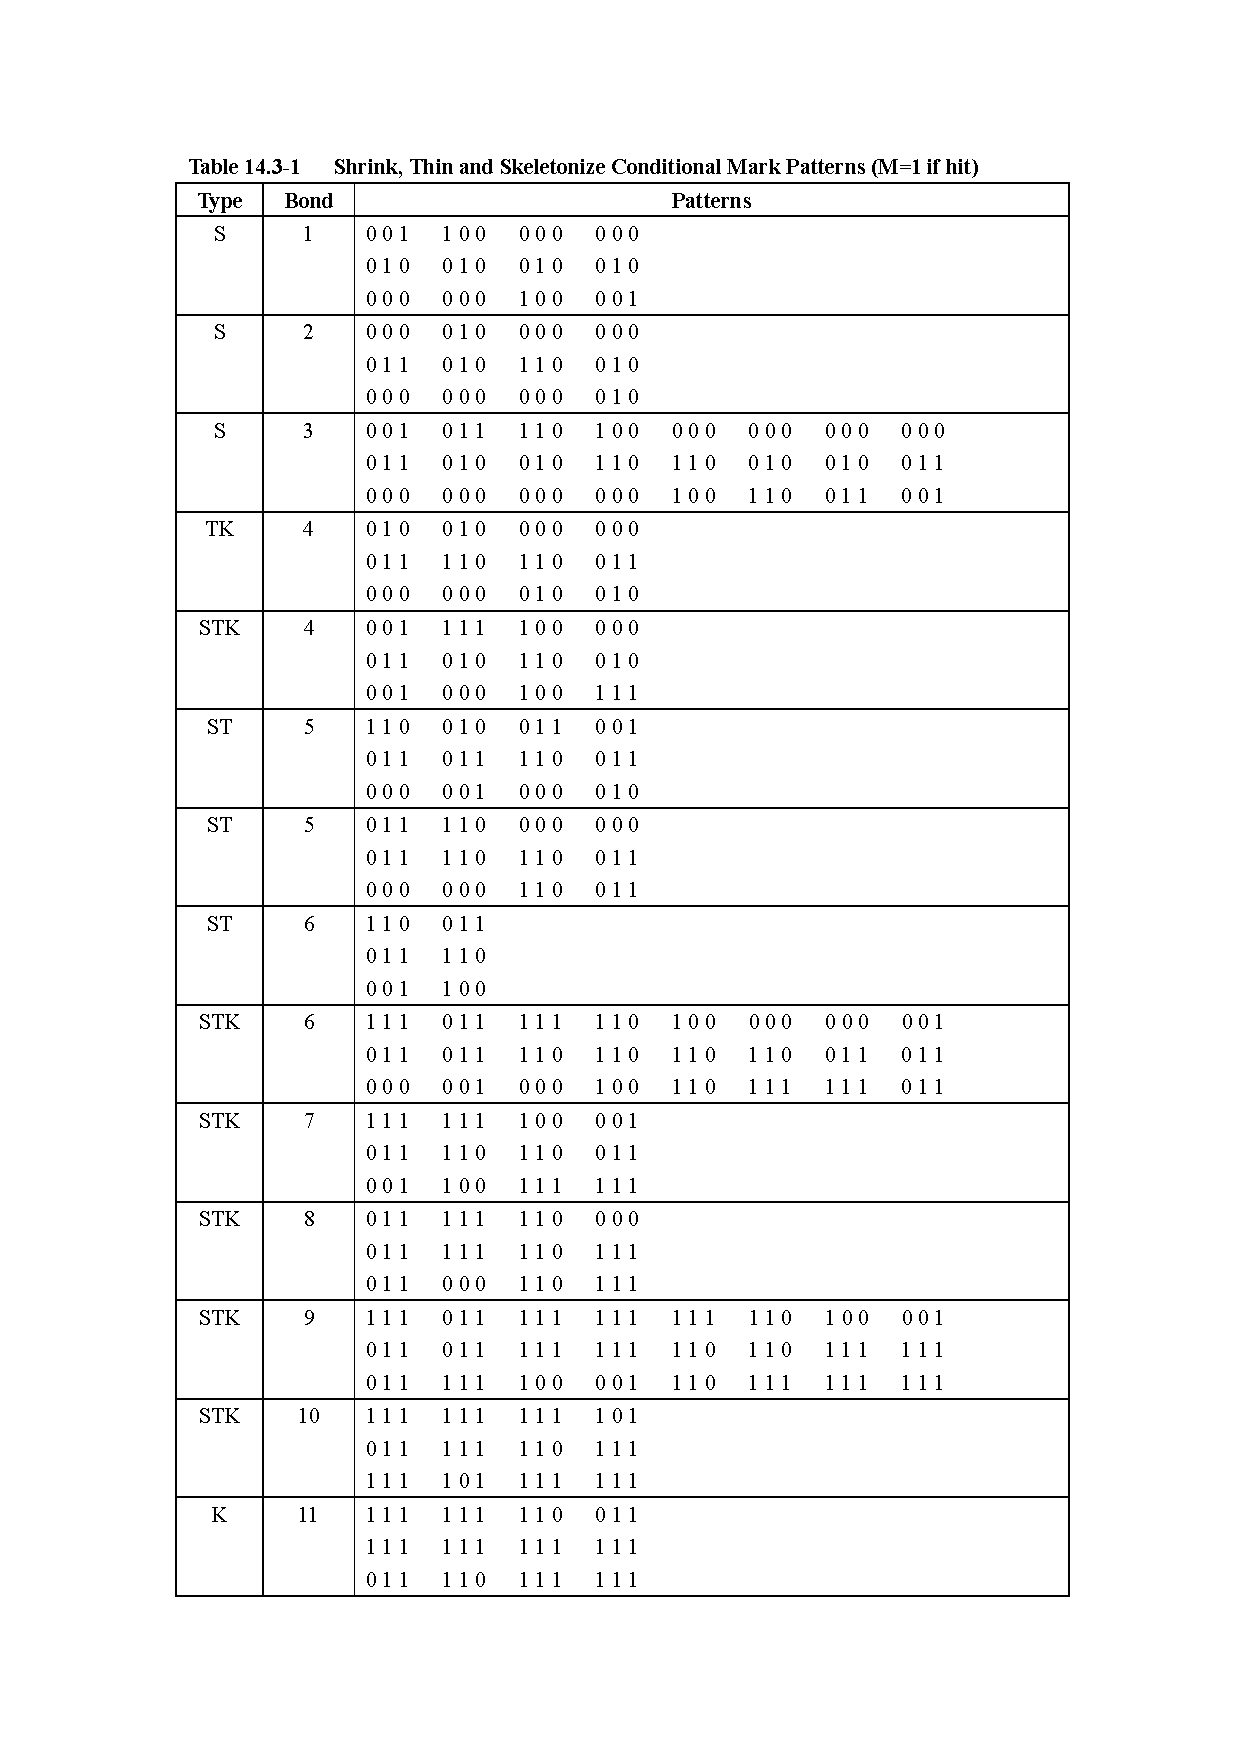
\includegraphics[page=1,height=19cm]{images/patternTables.pdf}
 \caption{Unconditional and Conditional Mark Patterns (part 1), taken from \cite{Pratt:2001:DIP:516234}, p. 413}
 \label{fig:markpatterns1}
\end{figure*}

\begin{figure*}[hb]
 \includegraphics[page=2,height=19cm]{images/patternTables.pdf}
 \caption{Unconditional and Conditional Mark Patterns (part 2), taken from \cite{Pratt:2001:DIP:516234}, p. 414}
 \label{fig:markpatterns2}
\end{figure*}

\begin{figure*}[hb]
 \includegraphics[page=3,height=19cm]{images/patternTables.pdf}
 \caption{Unconditional and Conditional Mark Patterns (part 3), taken from \cite{Pratt:2001:DIP:516234}, p. 415}
 \label{fig:markpatterns3}
\end{figure*}


\bibliography{report}
\bibliographystyle{plain}
\end{document}
